\section{Light from Planets}

When starlight reaches a planet, part of it is absorbed and converted into heat, while another part is returned to space without being thermalized. The former is re-emitted to space as thermal \emph{emission}. If the planet is young, internal heat contributes as well. The latter process returns photons more or less directly and is generally termed \emph{reflection/scattering}. Scattering stochastically redirects photons within the atmosphere, whereas reflection discretely changes the direction of propagation at the surface or cloud tops.

When considering light from exoplanets, one must properly account for the planetary sphericity. For emission, the intensity from the entire spherical surface must be considered, and for reflection, the relative geometry of the star, planet, and observer is crucial.

\begin{figure}[h]
\begin{center}
	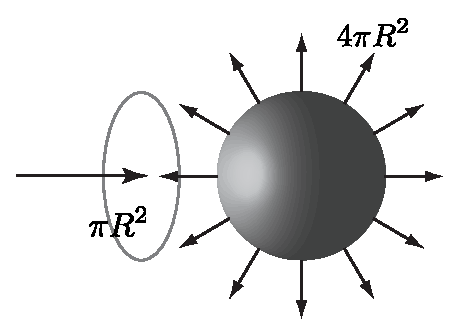
\includegraphics[width=\linewidth]{fig/io.eps}
\end{center}
\caption{Incident starlight onto a planet and thermal emission leaving the planetary surface.}
\label{fig:io}
\end{figure}

The energy received by a planet of radius $R$ can be written using the stellar flux density $S$ as
\begin{align}
\label{eq:lab}
L_{\mathrm{ab}}=(1-A) \pi R^2 S,
\end{align}
where $\pi R^2$ is the planetary cross section (see Fig.~\ref{fig:io}). Here $A$ is the planet-wide reflectivity (albedo), and the factor $(1-A)$ excludes the fraction reflected back to space. If the stellar radiation is approximated as blackbody emission, the stellar flux density is
\begin{align}
\label{eq:starfluxdens}
S= \frac{L_\star}{4 \pi a^2} = \frac{4 \pi R_\star^2 \sigma T_\star^4}{4 \pi a^2}\,\,\mathrm{W/m^2},
\end{align}
where $a$ is the orbital radius, $R_\star$ the stellar radius, $T_\star$ the stellar temperature, and $\sigma$ the Stefan--Boltzmann constant. For Earth, $S_\odot =1370 \,\mathrm{W/m^2}$ is called the solar constant.

If planetary emission is approximated as blackbody radiation at temperature $T_{\mathrm{eq}}$, the emitted power is
\begin{align}
\label{eq:lem}
L_{\mathrm{em}} = \beta \left( 4 \pi R^2 \sigma T_{\mathrm{eq}}^4 \right) + L_\mathrm{int},
\end{align}
where $L_\mathrm{int}$ is the planet's internal heat. For young planets this term can dominate, and such planets are referred to as self-luminous. The parameter $\beta$ characterizes the degree of heat redistribution: $\beta=1$ corresponds to instantaneous, uniform redistribution over the entire globe, while $\beta=0.5$ corresponds to redistribution over only the dayside hemisphere. This factor accounts for close-in, tidally locked planets whose same hemisphere always faces the star, as with the Moon relative to Earth.

For mature planets, internal emission can typically be neglected so that $L_\mathrm{int}=0$. In this case, the absorbed stellar energy should balance the emitted thermal energy,
\begin{align}
\label{eq:lemeqi}
L_{\mathrm{em}} = L_{\mathrm{ab}},
\end{align}
and the temperature $T_{\mathrm{eq}}$ satisfying this condition (radiative equilibrium) is called the \emph{equilibrium temperature}. Combining Eqs.~(\ref{eq:lab})--(\ref{eq:lemeqi}) yields
\begin{align}
\label{eq:eqteq}
\frac{T_{\mathrm{eq}}^4 a^2 }{T_\star^4 R_\star^2} = \frac{1-A}{4 \beta},
\end{align}
or
\begin{align}
&T_\mathrm{eq} = \left(\frac{1-A}{4 \beta}\right)^{\frac{1}{4}} T_\star \sqrt{\frac{R_\star}{a}} \\
&= 396 \,\mathrm{K}\, \left(\frac{1-A}{4 \beta}\right)^{\frac{1}{4}} \left( \frac{T_\star}{5800 \,\mathrm{K}}\right) \left( \frac{R_\star}{R_\odot}\right)^{\frac{1}{2}} \left( \frac{a}{1 \,\mathrm{au}}\right)^{-\frac{1}{2}} \\
&= 396 \,\mathrm{K}\, \left(\frac{1-A}{4 \beta}\right)^{\frac{1}{4}} \left( \frac{L_\star}{L_\odot}\right)^{\frac{1}{4}} \left( \frac{a}{1 \,\mathrm{au}}\right)^{-\frac{1}{2}}.
\end{align}

We also define the mean stellar flux received at the planetary surface. From Eq.~(\ref{eq:lab}),
\begin{align}
\label{eq:aveinpuF}
F_\star &\equiv \frac{L_{\mathrm{ab}}}{4 \pi R^2}= \frac{(1 - A)}{4} S \\
&= 240 \left(\frac{1-A}{0.7}\right) \left(\frac{S}{S_\odot}\right) \mathrm{W/m^2},
\end{align}
which relates directly to $S$. This expression represents the following picture: subtract the reflected fraction from the incident stellar energy, and multiply by the factor $1/4$ that accounts for redistribution by planetary rotation from the illuminated cross section (the disk in Fig.~\ref{fig:io}) over the full spherical surface. The mean absorbed flux density and the equilibrium temperature are related by
\begin{align}
\label{eq:teq}
\sigma T^4_{\mathrm{eq}} = F_\star/\beta.
\end{align}
\subsection*{Radiance and Irradiance}

From a distance, planets and stars appear as point sources, but on closer view they usually exhibit three-dimensional structures with continuous density variations. However, by considering a reference spherical surface --- for example, the planetary surface or the top of the atmosphere for Earth, or the photosphere for a star --- calculations become simpler if we describe radiation \emph{from} or \emph{onto} such a surface. To this end, let us first define quantities that allow us to quantify radiation from, or onto, a finite surface element.

Consider the energy $dE$ passing, per unit time and per unit wavelength, through a solid angle element $d\Omega$ (Fig.~\ref{fig:int}, top) in the direction ${\bf \Omega}$, emitted from an infinitesimal surface element $dA$. Here ${\bf n}$ denotes the unit normal vector. Since $dE$ is proportional to the apparent projected area $\cos{\theta} \, dA$, we can write
\begin{align}
d E = L_{\uparrow}(\theta,\phi) \cos{\theta} \, d A \, d \Omega \, d \nu,
\end{align}
where the proportionality factor $L_{\uparrow}$ is defined as the \emph{radiance}\index{Radiance@Radiance}. This allows us to define radiation independent of projection effects. Its units are, for example, [$\mathrm{W/m^2/sr/\mu m}$].

The net energy flux leaving $dA$ in the direction of ${\bf n}$ is called the \emph{irradiance}\index{Irradiance@Irradiance} $E_{\uparrow}$, given by
\begin{align}
E_{\uparrow} &= \int_{\mathrm{us}} dE = \int  d \Omega \, L_{\uparrow} (\theta,\phi) \cos{\theta} \\
\label{eq:rad}
&= \int_{0}^{2 \pi} d \phi  \int_{0}^{\pi/2} d \theta \, L_{\uparrow} (\theta,\phi) \cos{\theta} \sin{\theta},
\end{align}
where the integration is over the upper hemisphere (us).

\begin{figure}[]
\begin{center}
	\includegraphics[width=\linewidth]{fig/radiance_bw.png}
	\includegraphics[width=\linewidth]{fig/brdfdef_bw.png}
\end{center}
\caption{(Top) Radiation from or onto a surface element $dA$. (Bottom) Incidence of collimated light from direction $(\vartheta_0,\varphi_0)$ and reflection per unit solid angle $d\Omega$ into the same direction.}
\label{fig:int}
\end{figure}

\section{Emission Spectrum}

Let us consider the flux measured at a distance $d$ from a sphere of radius $R_p$ emitting blackbody radiation at temperature $T$. A surface with temperature $T$ emits blackbody radiation, whose radiance is
\begin{align}
L_{\uparrow} d \lambda = B_\lambda (T) d \lambda = \frac{2 h c^2}{\lambda^5} \frac{1}{\exp{(hc/\lambda k_B T)}-1} d \lambda.
\end{align}
Consider the radiation cone $d \Omega$ from a surface element $d A$, and let a telescope with aperture $d A_\mathrm{tel}$ located at distance $d$ be the tip of this cone ($d \Omega = d A_\mathrm{tel}/d^2$). The energy $\Delta E d A_\mathrm{tel}$ received by $d A_\mathrm{tel}$ from $d A$ is then
\begin{eqnarray}
\label{eq:brdfdef3}
\Delta E d A_\mathrm{tel} &=& L_\uparrow \cos{\vartheta_1} d \Omega d A \\
&=& \frac{L_\uparrow}{d^2} \cos{\vartheta_1} d A d A_\mathrm{tel}.
\end{eqnarray}
Thus, the irradiance or flux from the surface element $d A$ as seen by the observer is
\begin{eqnarray}
\label{eq:brdfdef6}
\Delta E = \frac{L_\uparrow}{d^2} \cos{\vartheta_1} d A.
\end{eqnarray}

Integrating over the entire sphere gives
\begin{align}
\label{eq:raddef}
f_p &= \int_\mathrm{planet} \Delta E = \int_\mathrm{planet} d A \frac{B_\nu (T)}{d^2} \cos{\vartheta_1} \\
&= R_p^2 B_\nu (T) \int_0^{2 \pi} d \varphi_1 \int_0^{\pi/2} d \vartheta_1 \sin{\vartheta_1} \cos{\vartheta_1}\\
&= \pi B_\nu (T) \frac{R_p^2}{d^2}.
\end{align}
The total luminosity is obtained by integrating over frequency and multiplying by the surface area of the sphere at distance $d$:
\begin{align}
\label{eq:raddeftot}
L &= 4 \pi d^2 \int_0^{\infty} d \nu \, \pi B_\nu (T) \frac{R_p^2}{d^2} = 4 \pi R_p^2 \sigma T^4.
\end{align}

\begin{itembox}{On the upward flux}
%\tiny
\footnotesize
\color{gray}
In radiative equilibrium models of planetary atmospheres, one typically considers the flux in a one-dimensional vertical column, often imposing the surface flux as a boundary condition. Similarly, let us consider the flux emitted upward from a blackbody surface element. Integrating over the upward hemisphere yields
\begin{align}
\label{eq:defsurf}
F_\nu (T) &= \Delta E = \int_\mathrm{us} d \Omega \, B_\nu (T) \cos{\vartheta_1} = \pi B_\nu (T).
\end{align}
The total flux is obtained by integrating over frequency:
\begin{align}
\label{eq:defsurflum}
F (T) &= \int d \nu \, f_\nu (T) = \sigma T^4.
\end{align}
\end{itembox}

To zeroth order, the emission spectrum of a planet can be approximated by blackbody radiation at a single temperature $T_p$:
\begin{align}
f_p (\lambda) d\, \lambda  &= \pi B_\lambda(\lambda,T_p) \frac{ R_p^2}{d^2}  d \lambda \\
&= \frac{2 \pi h c^2}{\lambda^5} \frac{ R_p^2}{d^2} \left[ \exp{ \left(\frac{h c}{\lambda k_B T_p} \right) }- 1 \right]^{-1} d\, \lambda ,
\label{eq:planckdist}
\end{align}
in some cases.

For example, the Earth's emission spectrum, with little atmospheric absorption, can be roughly approximated by blackbody radiation at surface temperatures $T=200$--$300$ K. However, for gas giants and brown dwarfs, the blackbody approximation is inadequate, primarily due to strong molecular absorption in their atmospheres. The observed spectrum is closer to the blackbody emission from atmospheric layers where the optical depth is near unity, which varies strongly with wavelength due to molecular absorption. These large deviations from blackbody emission are a characteristic signature of exoplanetary atmospheres.

\section{Reflection and Scattering Spectrum}

Reflected light is somewhat more complex because the observed intensity depends on the relative positions of the reflecting surface and the observer. However, on average, it can be treated as follows. In Eq.~(\ref{eq:lab}), the fraction of stellar energy not absorbed by the planet is reflected. Thus, the reflected luminosity is
\begin{align}
    L^\mathrm{ref}_p = A \pi R_p^2 S = \frac{L_\star}{4 \pi a^2} \pi R_p^2 A,
\end{align}
where $A$ is the planetary albedo. The mean reflected flux received at distance $d$ is
\begin{align}
    \langle f_{p}^\mathrm{ref} \rangle = \frac{ L^\mathrm{ref}_p}{4 \pi d^2}.
\end{align}
Using the stellar flux
\begin{align}
    f_\star = \frac{L_\star}{4 \pi d^2},
\end{align}
this can be written as
\begin{align}
    \langle f_{p}^\mathrm{ref} \rangle = \frac{A}{4} \left( \frac{R_p}{a} \right)^2 f_\star.
\end{align}

From a spectral perspective, the key point is that the wavelength dependence arises from the product $A(\lambda) f_\star(\lambda)$, i.e., the stellar spectrum modulated by the planetary reflection spectrum:
\begin{align}
    \langle f_{p}^\mathrm{ref} \rangle (\lambda) d \lambda = \frac{1}{4} \left( \frac{R_p}{a} \right)^2 A(\lambda) f_\star (\lambda) d \lambda.
\end{align}

Computing the flux as a function of orbital phase, rather than as a mean, is somewhat more involved and is omitted here (see Kawahara, \emph{Exoplanet Exploration}, Sec.~5.1.1). Here we simply summarize the result. The reflected flux $f_p^\mathrm{ref} (\lambda)$ observed at distance $d$ is expressed in terms of the star–planet separation $a$, the planetary albedo $A(\lambda)$, the planetary radius $R_p$, the observed stellar flux $f_\star(\lambda)$, and the phase function $\phi(\beta)$, which depends on the star–planet–observer phase angle $\beta$:
\begin{align}
\label{eq:refplanet}
f_p^\mathrm{ref} (\lambda) = \frac{2 \phi(\beta)}{3} A(\lambda) \left(\frac{R_p}{a}\right)^2 f_\star (\lambda),
\end{align}
\begin{align}
\label{eq:phaselambert}
\phi(\beta) \equiv [\sin{\beta} +  (\pi - \beta) \cos{\beta}]/\pi.
\end{align}
Here, $\phi(\beta)$ is the \emph{Lambert phase function}\index{Lambert phase function@Lambert phase function}, a function of the phase angle $\beta = \angle$(star–planet–observer). Note, however, that this relation assumes isotropic scattering. Strongly anisotropic processes, such as specular reflection from oceans (ocean glint), may not follow this approximation.

Although detection of reflected or scattered starlight from exoplanets is currently limited to specific cases such as precise space-based photometry of phase curves, in principle it is a rich source of information about the two-dimensional distribution of planetary surface and atmospheric properties. A key diagnostic in reflected light is the flux ratio between the star and the planet, known as the {\bf star–planet contrast}:
\begin{align}
\label{eq:contrast}
c_{\mathrm{sp}} (\lambda) \equiv \frac{f_p (\lambda)}{f_\star (\lambda)}.
\end{align}
A smaller contrast makes detection easier, both in direct imaging and in phase curve measurements.

For the half-phase geometry ($\beta = 90^\circ$), using Eq.~(\ref{eq:refplanet}), the star–planet contrast can be estimated. For Earth, we obtain
\begin{align}
\label{eq:refplanetearth}
c_\mathrm{sp}  \approx 10^{-10} \left( \frac{A}{0.3} \right) \left(\frac{R_p}{R_\oplus} \right)^{2} \left(\frac{a}{1 \, \mathrm{au}} \right)^{-2},
\end{align}
while for a hot Jupiter,
\begin{align}
\label{eq:refplanethj}
c_\mathrm{sp}  \approx 10^{-6} \left( \frac{A}{0.1} \right) \left(\frac{R_p}{R_J} \right)^{2} \left(\frac{a}{0.05 \, \mathrm{au}} \right)^{-2}.
\end{align}
